\documentclass[crop,tikz]{standalone}
\usepackage{pgfplots}

% http://pgfplots.net/tikz/examples/bell-curve/
\pgfplotsset{compat=1.8}
\pgfmathdeclarefunction{gauss}{2}{\pgfmathparse{1/(sqrt(#2*2*pi))*exp(-((x-#1)^2)/(2*#2))}}
\pgfmathdeclarefunction{multigauss}{4}{\pgfmathparse{1/(sqrt(#2*2*pi))*exp(-((x-#1)^2)/(2*#2)) * 1/(sqrt(#4*2*pi))*exp(-((y-#3)^2)/(2*#4))}}

\pgfplotsset{colormap={whiteblack}{color(0cm)=(white); color(1cm)=(gray)}}

\usetikzlibrary{positioning,shapes,arrows}

\begin{document}
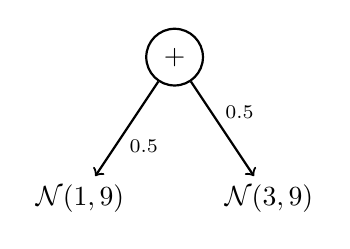
\begin{tikzpicture}
    [scale=.6,auto=left,every node/.style={inner sep = 3pt, minimum width = 0.72cm}]
  \node[draw, circle, thick] (n0) at (3,10) {$+$};
  \node[draw=none] (n1) at (1,7) {$\mathcal{N}(1, 9)$};
  \node[draw=none] (n2) at (5,7) {$\mathcal{N}(3, 9)$};

  \foreach \from/\to/\weight in {n0/n1/0.5, n0/n2/0.5}
    \draw (\from) edge[->, thick] node[draw=none, circle=none, minimum width=0.5cm, minimum height=0.2cm, inner sep=2pt]{\scriptsize \weight} (\to);
\end{tikzpicture}
\end{document}
